\chapter{Madame de Saint-Méran}

A gloomy scene had indeed just passed at the house of M. de Villefort.
After the ladies had departed for the ball, whither all the entreaties
of Madame de Villefort had failed in persuading him to accompany them,
the procureur had shut himself up in his study, according to his
custom, with a heap of papers calculated to alarm anyone else, but
which generally scarcely satisfied his inordinate desires.

But this time the papers were a mere matter of form. Villefort had
secluded himself, not to study, but to reflect; and with the door
locked and orders given that he should not be disturbed excepting for
important business, he sat down in his armchair and began to ponder
over the events, the remembrance of which had during the last eight
days filled his mind with so many gloomy thoughts and bitter
recollections.

Then, instead of plunging into the mass of documents piled before him,
he opened the drawer of his desk, touched a spring, and drew out a
parcel of cherished memoranda, amongst which he had carefully arranged,
in characters only known to himself, the names of all those who, either
in his political career, in money matters, at the bar, or in his
mysterious love affairs, had become his enemies.

Their number was formidable, now that he had begun to fear, and yet
these names, powerful though they were, had often caused him to smile
with the same kind of satisfaction experienced by a traveller who from
the summit of a mountain beholds at his feet the craggy eminences, the
almost impassable paths, and the fearful chasms, through which he has
so perilously climbed. When he had run over all these names in his
memory, again read and studied them, commenting meanwhile upon his
lists, he shook his head.

“No,” he murmured, “none of my enemies would have waited so patiently
and laboriously for so long a space of time, that they might now come
and crush me with this secret. Sometimes, as Hamlet says:

\begin{quote}
{\small‘Foul deeds will rise,

Though all the earth o’erwhelm them, to men’s eyes;’}
\end{quote}

but, like a phosphoric light, they rise but to mislead. The story has
been told by the Corsican to some priest, who in his turn has repeated
it. M. de Monte Cristo may have heard it, and to enlighten himself——

“But why should he wish to enlighten himself upon the subject?” asked
Villefort, after a moment’s reflection, “what interest can this M. de
Monte Cristo or M. Zaccone,—son of a shipowner of Malta, discoverer of
a mine in Thessaly, now visiting Paris for the first time,—what
interest, I say, can he take in discovering a gloomy, mysterious, and
useless fact like this? However, among all the incoherent details given
to me by the Abbé Busoni and by Lord Wilmore, by that friend and that
enemy, one thing appears certain and clear in my opinion—that in no
period, in no case, in no circumstance, could there have been any
contact between him and me.”

But Villefort uttered words which even he himself did not believe. He
dreaded not so much the revelation, for he could reply to or deny its
truth;—he cared little for that \textit{mene, mene, tekel upharsin}, which
appeared suddenly in letters of blood upon the wall;—but what he was
really anxious for was to discover whose hand had traced them. While he
was endeavoring to calm his fears,—and instead of dwelling upon the
political future that had so often been the subject of his ambitious
dreams, was imagining a future limited to the enjoyments of home, in
fear of awakening the enemy that had so long slept,—the noise of a
carriage sounded in the yard, then he heard the steps of an aged person
ascending the stairs, followed by tears and lamentations, such as
servants always give vent to when they wish to appear interested in
their master’s grief.

He drew back the bolt of his door, and almost directly an old lady
entered, unannounced, carrying her shawl on her arm, and her bonnet in
her hand. The white hair was thrown back from her yellow forehead, and
her eyes, already sunken by the furrows of age, now almost disappeared
beneath the eyelids swollen with grief.

“Oh, sir,” she said; “oh, sir, what a misfortune! I shall die of it;
oh, yes, I shall certainly die of it!”

And then, falling upon the chair nearest the door, she burst into a
paroxysm of sobs. The servants, standing in the doorway, not daring to
approach nearer, were looking at Noirtier’s old servant, who had heard
the noise from his master’s room, and run there also, remaining behind
the others. Villefort rose, and ran towards his mother-in-law, for it
was she.

“Why, what can have happened?” he exclaimed, “what has thus disturbed
you? Is M. de Saint-Méran with you?”

“M. de Saint-Méran is dead,” answered the old marchioness, without
preface and without expression; she appeared to be stupefied. Villefort
drew back, and clasping his hands together, exclaimed:

“Dead!—so suddenly?”

“A week ago,” continued Madame de Saint-Méran, “we went out together in
the carriage after dinner. M. de Saint-Méran had been unwell for some
days; still, the idea of seeing our dear Valentine again inspired him
with courage, and notwithstanding his illness he would leave. At six
leagues from Marseilles, after having eaten some of the lozenges he is
accustomed to take, he fell into such a deep sleep, that it appeared to
me unnatural; still I hesitated to wake him, although I fancied that
his face was flushed, and that the veins of his temples throbbed more
violently than usual. However, as it became dark, and I could no longer
see, I fell asleep; I was soon aroused by a piercing shriek, as from a
person suffering in his dreams, and he suddenly threw his head back
violently. I called the valet, I stopped the postilion, I spoke to M.
de Saint-Méran, I applied my smelling-salts; but all was over, and I
arrived at Aix by the side of a corpse.”

Villefort stood with his mouth half open, quite stupefied.

“Of course you sent for a doctor?”

“Immediately; but, as I have told you, it was too late.”

“Yes; but then he could tell of what complaint the poor marquis had
died.”

“Oh, yes, sir, he told me; it appears to have been an apoplectic
stroke.”

“And what did you do then?”

“M. de Saint-Méran had always expressed a desire, in case his death
happened during his absence from Paris, that his body might be brought
to the family vault. I had him put into a leaden coffin, and I am
preceding him by a few days.”

“Oh! my poor mother!” said Villefort, “to have such duties to perform
at your age after such a blow!”

“God has supported me through all; and then, my dear marquis, he would
certainly have done everything for me that I performed for him. It is
true that since I left him, I seem to have lost my senses. I cannot
cry; at my age they say that we have no more tears,—still I think that
when one is in trouble one should have the power of weeping. Where is
Valentine, sir? It is on her account I am here; I wish to see
Valentine.”

\begin{figure}[ht]
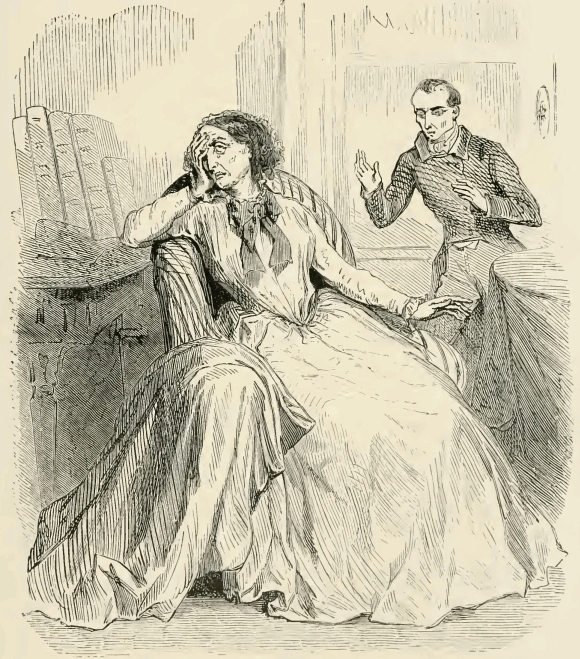
\includegraphics[width=\textwidth]{30315m.jpg}
\end{figure}

Villefort thought it would be terrible to reply that Valentine was at a
ball; so he only said that she had gone out with her step-mother, and
that she should be fetched. “This instant, sir—this instant, I beseech
you!” said the old lady. Villefort placed the arm of Madame de
Saint-Méran within his own, and conducted her to his apartment.

“Rest yourself, mother,” he said.

The marchioness raised her head at this word, and beholding the man who
so forcibly reminded her of her deeply-regretted child, who still lived
for her in Valentine, she felt touched at the name of mother, and
bursting into tears, she fell on her knees before an armchair, where
she buried her venerable head. Villefort left her to the care of the
women, while old Barrois ran, half-scared, to his master; for nothing
frightens old people so much as when death relaxes its vigilance over
them for a moment in order to strike some other old person. Then, while
Madame de Saint-Méran remained on her knees, praying fervently,
Villefort sent for a cab, and went himself to fetch his wife and
daughter from Madame de Morcerf’s. He was so pale when he appeared at
the door of the ball-room, that Valentine ran to him, saying:

“Oh, father, some misfortune has happened!”

“Your grandmamma has just arrived, Valentine,” said M. de Villefort.

“And grandpapa?” inquired the young girl, trembling with apprehension.
M. de Villefort only replied by offering his arm to his daughter. It
was just in time, for Valentine’s head swam, and she staggered; Madame
de Villefort instantly hastened to her assistance, and aided her
husband in dragging her to the carriage, saying:

“What a singular event! Who could have thought it? Ah, yes, it is
indeed strange!”

And the wretched family departed, leaving a cloud of sadness hanging
over the rest of the evening. At the foot of the stairs, Valentine
found Barrois awaiting her.

“M. Noirtier wishes to see you tonight, he said, in an undertone.

“Tell him I will come when I leave my dear grandmamma,” she replied,
feeling, with true delicacy, that the person to whom she could be of
the most service just then was Madame de Saint-Méran.

Valentine found her grandmother in bed; silent caresses, heartwrung
sobs, broken sighs, burning tears, were all that passed in this sad
interview, while Madame de Villefort, leaning on her husband’s arm,
maintained all outward forms of respect, at least towards the poor
widow. She soon whispered to her husband:

“I think it would be better for me to retire, with your permission, for
the sight of me appears still to afflict your mother-in-law.” Madame de
Saint-Méran heard her.

“Yes, yes,” she said softly to Valentine, “let her leave; but do you
stay.”

Madame de Villefort left, and Valentine remained alone beside the bed,
for the procureur, overcome with astonishment at the unexpected death,
had followed his wife. Meanwhile, Barrois had returned for the first
time to old Noirtier, who having heard the noise in the house, had, as
we have said, sent his old servant to inquire the cause; on his return,
his quick intelligent eye interrogated the messenger.

“Alas, sir,” exclaimed Barrois, “a great misfortune has happened.
Madame de Saint-Méran has arrived, and her husband is dead!”

M. de Saint-Méran and Noirtier had never been on strict terms of
friendship; still, the death of one old man always considerably affects
another. Noirtier let his head fall upon his chest, apparently
overwhelmed and thoughtful; then he closed one eye, in token of
inquiry.

Barrois asked, “Mademoiselle Valentine?”

Noirtier nodded his head.

“She is at the ball, as you know, since she came to say good-bye to you
in full dress.” Noirtier again closed his left eye.

“Do you wish to see her?” Noirtier again made an affirmative sign.

“Well, they have gone to fetch her, no doubt, from Madame de Morcerf’s;
I will await her return, and beg her to come up here. Is that what you
wish for?”

“Yes,” replied the invalid.

Barrois, therefore, as we have seen, watched for Valentine, and
informed her of her grandfather’s wish. Consequently, Valentine came up
to Noirtier, on leaving Madame de Saint-Méran, who in the midst of her
grief had at last yielded to fatigue and fallen into a feverish sleep.
Within reach of her hand they placed a small table upon which stood a
bottle of orangeade, her usual beverage, and a glass. Then, as we have
said, the young girl left the bedside to see M. Noirtier.

Valentine kissed the old man, who looked at her with such tenderness
that her eyes again filled with tears, whose sources he thought must be
exhausted. The old gentleman continued to dwell upon her with the same
expression.

“Yes, yes,” said Valentine, “you mean that I have yet a kind
grandfather left, do you not.” The old man intimated that such was his
meaning. “Ah, yes, happily I have,” replied Valentine. “Without that,
what would become of me?”

It was one o’clock in the morning. Barrois, who wished to go to bed
himself, observed that after such sad events everyone stood in need of
rest. Noirtier would not say that the only rest he needed was to see
his child, but wished her good-night, for grief and fatigue had made
her appear quite ill.

The next morning she found her grandmother in bed; the fever had not
abated, on the contrary her eyes glistened and she appeared to be
suffering from violent nervous irritability.

“Oh, dear grandmamma, are you worse?” exclaimed Valentine, perceiving
all these signs of agitation.

“No, my child, no,” said Madame de Saint-Méran; “but I was impatiently
waiting for your arrival, that I might send for your father.”

“My father?” inquired Valentine, uneasily.

“Yes, I wish to speak to him.”

Valentine durst not oppose her grandmother’s wish, the cause of which
she did not know, and an instant afterwards Villefort entered.

“Sir,” said Madame de Saint-Méran, without using any circumlocution,
and as if fearing she had no time to lose, “you wrote to me concerning
the marriage of this child?”

“Yes, madame,” replied Villefort, “it is not only projected but
arranged.”

“Your intended son-in-law is named M. Franz d’Épinay?”

“Yes, madame.”

“Is he not the son of General d’Épinay who was on our side, and who was
assassinated some days before the usurper returned from the Island of
Elba?”

“The same.”

“Does he not dislike the idea of marrying the granddaughter of a
Jacobin?”

“Our civil dissensions are now happily extinguished, mother,” said
Villefort; “M. d’Épinay was quite a child when his father died, he
knows very little of M. Noirtier, and will meet him, if not with
pleasure, at least with indifference.”

“Is it a suitable match?”

“In every respect.”

“And the young man?”

“Is regarded with universal esteem.”

“You approve of him?”

“He is one of the most well-bred young men I know.”

During the whole of this conversation Valentine had remained silent.

“Well, sir,” said Madame de Saint-Méran, after a few minutes’
reflection, “I must hasten the marriage, for I have but a short time to
live.”

“You, madame?” “You, dear mamma?” exclaimed M. de Villefort and
Valentine at the same time.

“I know what I am saying,” continued the marchioness; “I must hurry
you, so that, as she has no mother, she may at least have a grandmother
to bless her marriage. I am all that is left to her belonging to my
poor Renée, whom you have so soon forgotten, sir.”

“Ah, madame,” said Villefort, “you forget that I was obliged to give a
mother to my child.”

“A stepmother is never a mother, sir. But this is not to the
purpose,—our business concerns Valentine, let us leave the dead in
peace.”

All this was said with such exceeding rapidity, that there was
something in the conversation that seemed like the beginning of
delirium.

“It shall be as you wish, madame,” said Villefort; “more especially
since your wishes coincide with mine, and as soon as M. d’Épinay
arrives in Paris——”

\begin{figure}[ht]
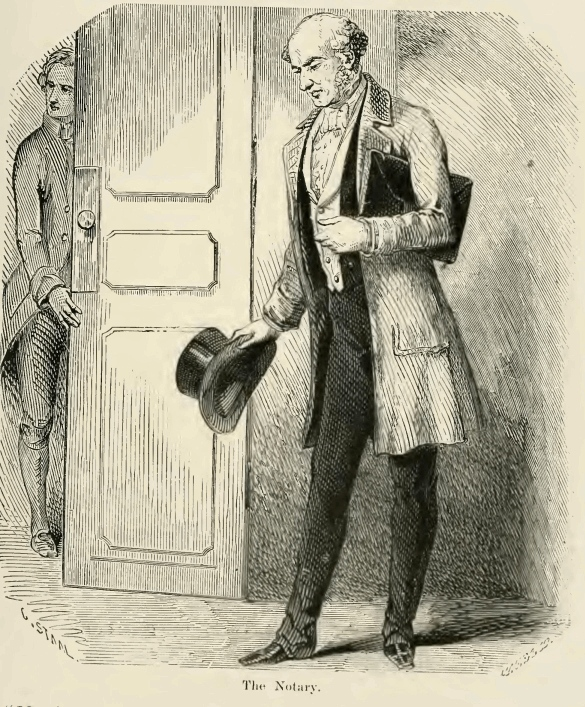
\includegraphics[width=\textwidth]{30319m.jpg}
\end{figure}

“My dear grandmother,” interrupted Valentine, “consider decorum—the
recent death. You would not have me marry under such sad auspices?”

“My child,” exclaimed the old lady sharply, “let us hear none of the
conventional objections that deter weak minds from preparing for the
future. I also was married at the death-bed of my mother, and certainly
I have not been less happy on that account.”

“Still that idea of death, madame,” said Villefort.

“Still?—Always! I tell you I am going to die—do you understand? Well,
before dying, I wish to see my son-in-law. I wish to tell him to make
my child happy; I wish to read in his eyes whether he intends to obey
me;—in fact, I will know him—I will!” continued the old lady, with a
fearful expression, “that I may rise from the depths of my grave to
find him, if he should not fulfil his duty!”

“Madame,” said Villefort, “you must lay aside these exalted ideas,
which almost assume the appearance of madness. The dead, once buried in
their graves, rise no more.”

“And I tell you, sir, that you are mistaken. This night I have had a
fearful sleep. It seemed as though my soul were already hovering over
my body, my eyes, which I tried to open, closed against my will, and
what will appear impossible above all to you, sir, I saw, with my eyes
shut, in the spot where you are now standing, issuing from that corner
where there is a door leading into Madame Villefort’s dressing-room—I
saw, I tell you, silently enter, a white figure.”

Valentine screamed.

“It was the fever that disturbed you, madame,” said Villefort.

\begin{figure}[ht]
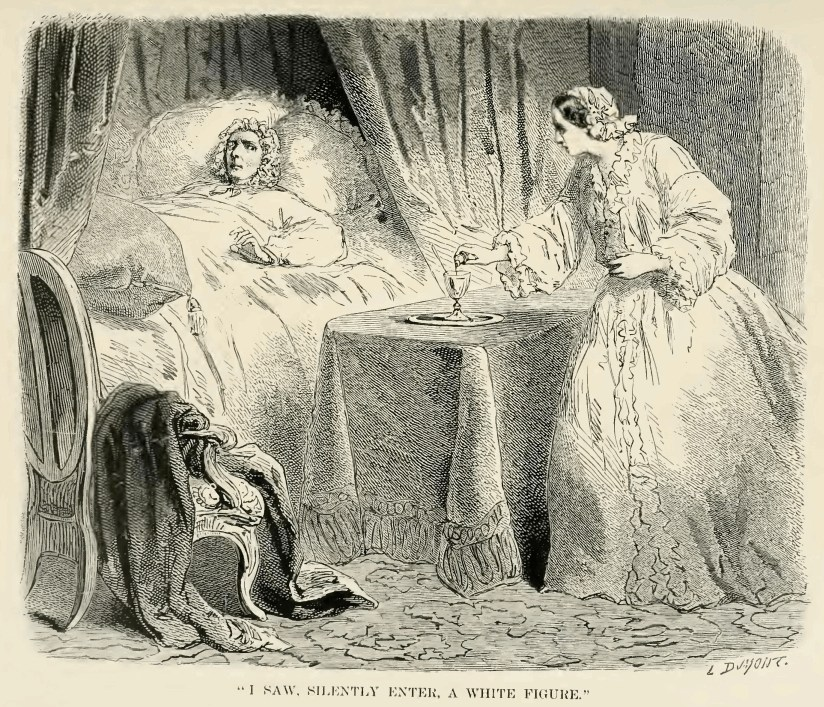
\includegraphics[width=\textwidth]{30321m.jpg}
\end{figure}

“Doubt, if you please, but I am sure of what I say. I saw a white
figure, and as if to prevent my discrediting the testimony of only one
of my senses, I heard my glass removed—the same which is there now on
the table.”

“Oh, dear mother, it was a dream.”

“So little was it a dream, that I stretched my hand towards the bell;
but when I did so, the shade disappeared; my maid then entered with a
light.”

“But she saw no one?”

“Phantoms are visible to those only who ought to see them. It was the
soul of my husband!—Well, if my husband’s soul can come to me, why
should not my soul reappear to guard my granddaughter? the tie is even
more direct, it seems to me.”

“Oh, madame,” said Villefort, deeply affected, in spite of himself, “do
not yield to those gloomy thoughts; you will long live with us, happy,
loved, and honored, and we will make you forget——”

“Never, never, never,” said the marchioness. “When does M. d’Épinay
return?”

“We expect him every moment.”

“It is well. As soon as he arrives inform me. We must be expeditious.
And then I also wish to see a notary, that I may be assured that all
our property returns to Valentine.”

“Ah, grandmamma,” murmured Valentine, pressing her lips on the burning
brow, “do you wish to kill me? Oh, how feverish you are; we must not
send for a notary, but for a doctor!”

“A doctor?” said she, shrugging her shoulders, “I am not ill; I am
thirsty—that is all.”

\begin{figure}[ht]
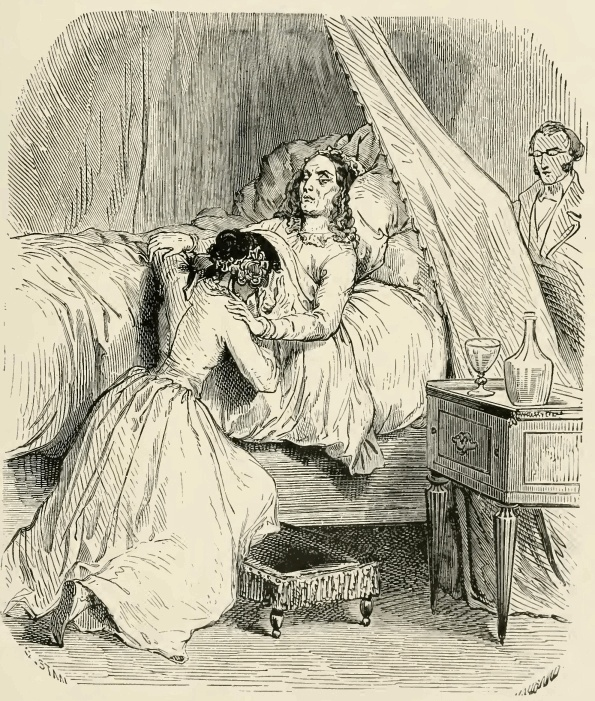
\includegraphics[width=\textwidth]{30323m.jpg}
\end{figure}

“What are you drinking, dear grandmamma?”

“The same as usual, my dear, my glass is there on the table—give it to
me, Valentine.” Valentine poured the orangeade into a glass and gave it
to her grandmother with a certain degree of dread, for it was the same
glass she fancied that had been touched by the spectre.

The marchioness drained the glass at a single draught, and then turned
on her pillow, repeating,

“The notary, the notary!”

M. de Villefort left the room, and Valentine seated herself at the
bedside of her grandmother. The poor child appeared herself to require
the doctor she had recommended to her aged relative. A bright spot
burned in either cheek, her respiration was short and difficult, and
her pulse beat with feverish excitement. She was thinking of the
despair of Maximilian, when he should be informed that Madame de
Saint-Méran, instead of being an ally, was unconsciously acting as his
enemy.

More than once she thought of revealing all to her grandmother, and she
would not have hesitated a moment, if Maximilian Morrel had been named
Albert de Morcerf or Raoul de Château-Renaud; but Morrel was of
plebeian extraction, and Valentine knew how the haughty Marquise de
Saint-Méran despised all who were not noble. Her secret had each time
been repressed when she was about to reveal it, by the sad conviction
that it would be useless to do so; for, were it once discovered by her
father and mother, all would be lost.

Two hours passed thus; Madame de Saint-Méran was in a feverish sleep,
and the notary had arrived. Though his coming was announced in a very
low tone, Madame de Saint-Méran arose from her pillow.

“The notary!” she exclaimed, “let him come in.”

The notary, who was at the door, immediately entered. “Go, Valentine,”
said Madame de Saint-Méran, “and leave me with this gentleman.”

“But, grandmamma——”

“Leave me—go!”

The young girl kissed her grandmother, and left with her handkerchief
to her eyes; at the door she found the valet de chambre, who told her
that the doctor was waiting in the dining-room. Valentine instantly ran
down. The doctor was a friend of the family, and at the same time one
of the cleverest men of the day, and very fond of Valentine, whose
birth he had witnessed. He had himself a daughter about her age, but
whose life was one continued source of anxiety and fear to him from her
mother having been consumptive.

“Oh,” said Valentine, “we have been waiting for you with such
impatience, dear M. d’Avrigny. But, first of all, how are Madeleine and
Antoinette?”

Madeleine was the daughter of M. d’Avrigny, and Antoinette his niece.
M. d’Avrigny smiled sadly.

“Antoinette is very well,” he said, “and Madeleine tolerably so. But
you sent for me, my dear child. It is not your father or Madame de
Villefort who is ill. As for you, although we doctors cannot divest our
patients of nerves, I fancy you have no further need of me than to
recommend you not to allow your imagination to take too wide a field.”

Valentine colored. M. d’Avrigny carried the science of divination
almost to a miraculous extent, for he was one of the physicians who
always work upon the body through the mind.

\begin{figure}[ht]
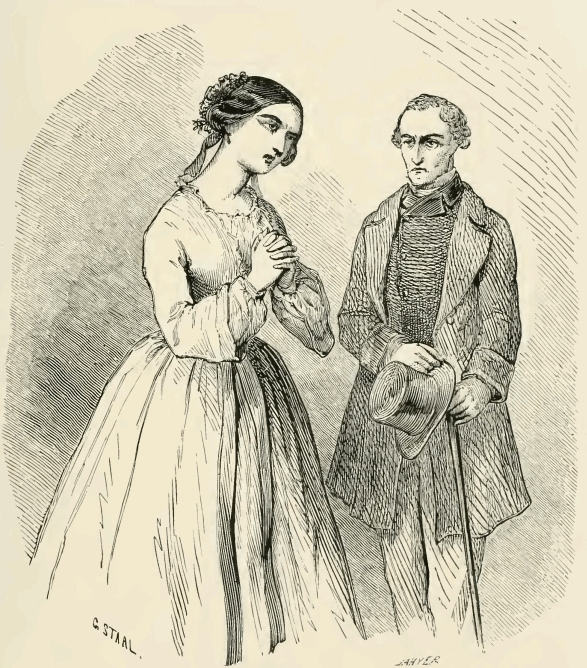
\includegraphics[width=\textwidth]{30325m.jpg}
\end{figure}

“No,” she replied, “it is for my poor grandmother. You know the
calamity that has happened to us, do you not?”

“I know nothing.” said M. d’Avrigny.

“Alas,” said Valentine, restraining her tears, “my grandfather is
dead.”

“M. de Saint-Méran?”

“Yes.”

“Suddenly?”

“From an apoplectic stroke.”

“An apoplectic stroke?” repeated the doctor.

“Yes, and my poor grandmother fancies that her husband, whom she never
left, has called her, and that she must go and join him. Oh, M.
d’Avrigny, I beseech you, do something for her!”

“Where is she?”

“In her room with the notary.”

“And M. Noirtier?”

“Just as he was, his mind perfectly clear, but the same incapability of
moving or speaking.”

“And the same love for you—eh, my dear child?”

“Yes,” said Valentine, “he was very fond of me.”

“Who does not love you?” Valentine smiled sadly. “What are your
grandmother’s symptoms?”

“An extreme nervous excitement and a strangely agitated sleep; she
fancied this morning in her sleep that her soul was hovering above her
body, which she at the same time watched. It must have been delirium;
she fancies, too, that she saw a phantom enter her chamber and even
heard the noise it made on touching her glass.”

“It is singular,” said the doctor; “I was not aware that Madame de
Saint-Méran was subject to such hallucinations.”

“It is the first time I ever saw her in this condition,” said
Valentine; “and this morning she frightened me so that I thought her
mad; and my father, who you know is a strong-minded man, himself
appeared deeply impressed.”

“We will go and see,” said the doctor; “what you tell me seems very
strange.” The notary here descended, and Valentine was informed that
her grandmother was alone.

“Go upstairs,” she said to the doctor.

“And you?”

“Oh, I dare not—she forbade my sending for you; and, as you say, I am
myself agitated, feverish and out of sorts. I will go and take a turn
in the garden to recover myself.”

The doctor pressed Valentine’s hand, and while he visited her
grandmother, she descended the steps. We need not say which portion of
the garden was her favorite walk. After remaining for a short time in
the parterre surrounding the house, and gathering a rose to place in
her waist or hair, she turned into the dark avenue which led to the
bench; then from the bench she went to the gate. As usual, Valentine
strolled for a short time among her flowers, but without gathering
them. The mourning in her heart forbade her assuming this simple
ornament, though she had not yet had time to put on the outward
semblance of woe.

\begin{figure}[ht]
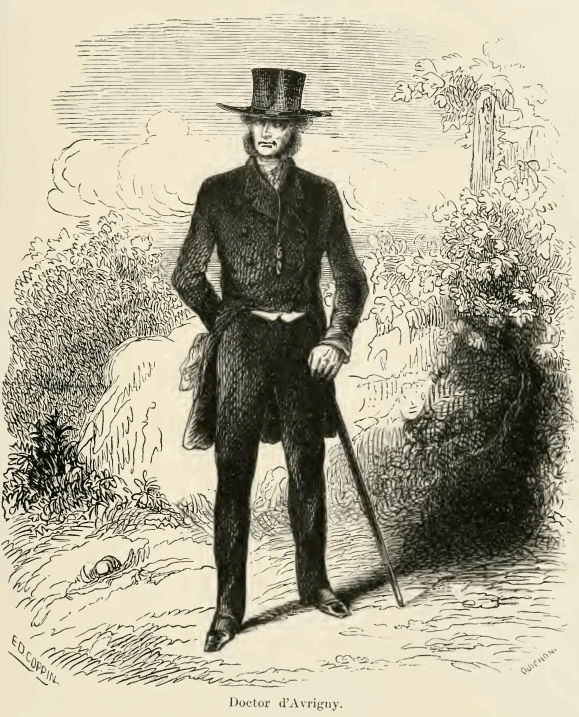
\includegraphics[width=\textwidth]{30327m.jpg}
\end{figure}

She then turned towards the avenue. As she advanced she fancied she
heard a voice speaking her name. She stopped astonished, then the voice
reached her ear more distinctly, and she recognized it to be that of
Maximilian.
